% !TeX program = pdflatex

\documentclass[11pt, conference]{IEEEtran}
\usepackage{hyperref}
\hypersetup{unicode, bookmarksnumbered, bookmarksopen, breaklinks, hidelinks, pdfstartview=FitH}
\AtBeginDocument{\urlstyle{tt}}
\usepackage{amsmath, amsfonts, amssymb}
\usepackage{txfonts}
\usepackage{graphicx, xcolor}
\graphicspath{{figures/}}
\usepackage{cite}
\usepackage{booktabs}
%\usepackage{subcaption}
\usepackage{float}
\newcommand{\tcr}{\textcolor{red}}

\let\Mean\overline
\def\D{\mathrm{d}}
\def\Email#1{\href{mailto:#1@shanghaitech.edu.cn}{#1}}

\begin{document}

\title{CS120 Project : Athernet}
\author{%
\IEEEauthorblockN{Hongdi Yang \qquad Yibo Zhao}
\IEEEauthorblockA{ShanghaiTech University \\
\texttt{\char`\{\Email{yanghd}, \Email{zhaoyb1}\char`\}@shanghaitech.edu.cn}}
}
\maketitle

\section{Introduction}

As the project for CS120, We implement Athernet, a toy net that uses acoustic signal or sound to transmit information through the 
audio connection. We implemented the physical layer and MAC layer of the network. We also implemented a NAT for
Athernet to make it communicate with internet. Last, we implemented an FTP client for Athernet nodes on UDP protocol so we can download files 
for the off-net Athernet node via the audio connection. In this project, we use C++ for Athernet implementation and use python to
implement part of NAT for Internet transmission.

\section{Project 1: Acoustic Connection}

In this project, we work on physical layer of Athernet. We choose ASIO, a computer sound card driver protocol for digital audio that provides a low-latency and high fidelity
interface between a software application and a computer's sound card to generate and receive sound wave, and develop our project based 
on JUCE, a C++ application framework which provides powerful support for audio transmission. We encode the transferring bitstream as samples 
of sound wave by PSK method, packed with header wave as a physical layer frame. As a result, we successfully transmit 10000 bits by our own microphone and speaker in 15 seconds
with accuracy of 100 percent. However, the transmission is fragile and susceptible to noise from surrounding.

\subsection{Modulation}

We choose PSK to modulate bitstream. In original design (without OFDM), we use the wave $1 \times cos(2\pi \times 5000 x)$ to represent 1, and
$  1 \times cos(2\pi \times 5000 x + \pi) = -cos(2\pi \times 5000 x)$ to represent 0. We choose the sample rate of 48000Hz, and by fully test the hardware, 
we find that 400 bits per frame and 48 samples per bit best fit our devices, giving consideration of both accuracy and bandwidth.

As for header wave, it is also a sin wave that start with frequency 200Hz, and continuously increases its frequency until 10000Hz, and after that, its
frequency decreases at the same speed to 2000Hz, which is shown in Fig.1

\begin{figure}[!h]
	\centering
	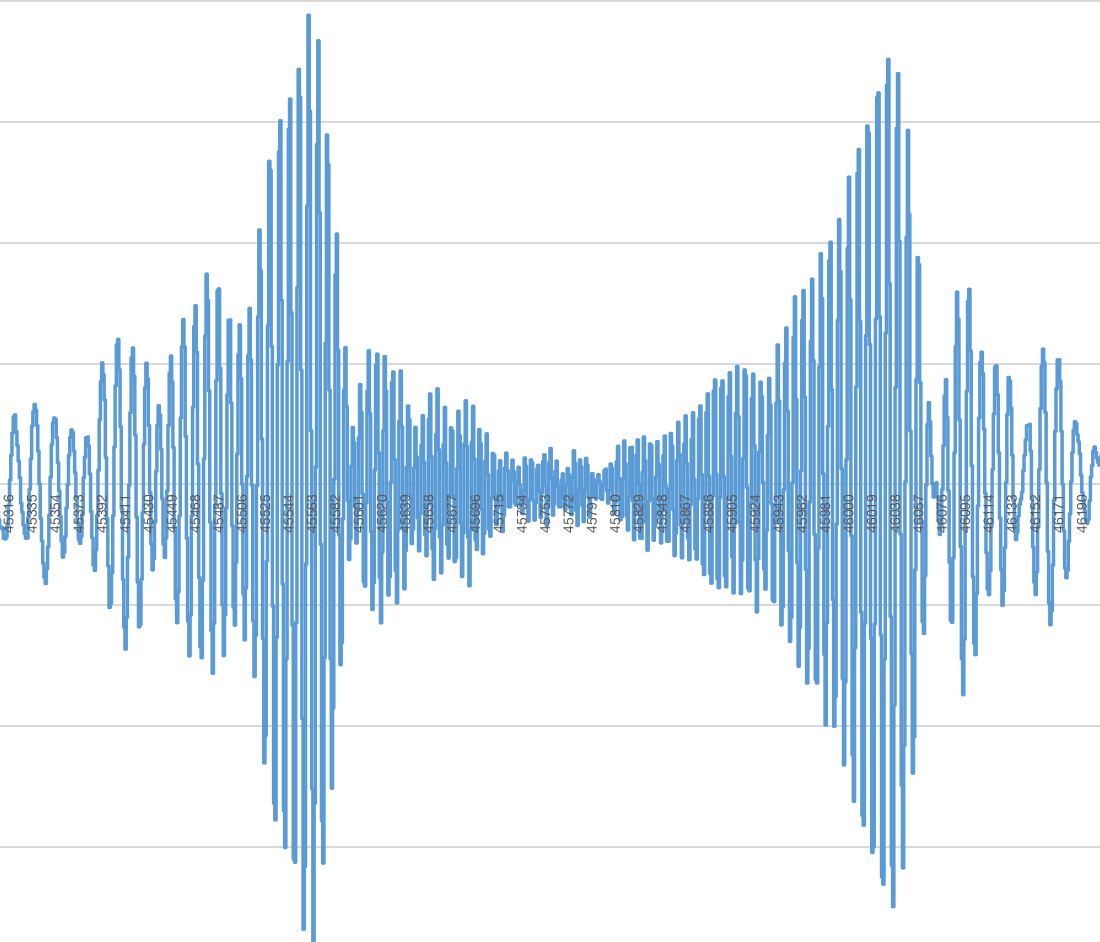
\includegraphics[scale=0.4]{header_wave.png}
	\caption{header wave}\label{}
	\end{figure}

\subsection{{Demodulation}}
    For demodulation, we have two states for processing the audio samples: the header synchronization state and the data processing state.
\subsubsection{Header Synchronization State}
    In header synchronization state, we first wait until enough samples arrive(i.e. the length of the pre-defined header). Once we get enough samples, we use the \textbf{SyncPower}
    to detect the header. We define $$SyncPower = \sum_{i}^{Headerlength} Header[i] \cdot Samples[i]$$
    so that the SyncPower will be the largest when the header is detected(as for every $i$, $Header[i] = Samples[i]$).

    Considering possible noises, we also use \textbf{ChannelPower} to detect the local power in channels. We define
    $$ChannelPower = ChannelPower\cdot (1 - \frac{1}{64}) + sample^2 \cdot \frac{1}{64}$$
    which gives an approximate current power in channels. And we will only accept the header if the \textbf{SyncPower} > \textbf{ChannelPower}.

    Once we detect the header, we will also wait for another 500 samples to make sure the \textbf{SyncPower} we find is the largest, indicating the header found is correct.
\subsubsection{Data Processing State}
    In data processing state, we first decode the length field to know how many samples we need to process the data.
    Then we wait until enough samples arrive.

    Once we get enough samples, we start to decode every bit. As in Modulation, we use the wave $1 \times cos(2\pi \times 5000 x)$ to represent 1, and
    $  1 \times cos(2\pi \times 5000 x + \pi) = -cos(2\pi \times 5000 x)$ to represent 0. Then we calculate 
    $$bitsum = \sum_{i}^{N}cos(\frac{2\pi \times 5000 i}{sampleRate}) \cdot bitsamples[i] $$
    where $N$ is the number of samples per bit. And if the bit we receive is 1, $bitsum$ should be positive. If the bit we receive is 0, then the $bitsum$
    should be negative.

    After processing all bits we receive, we get the data from the sender now.
\subsection{Higher bandwidth: OFDM}

OFDM is a method to encode bits on multiple carrier frequencies. 'O' is orthogonal, and if we use two or more sin waves to transmit simultaneously,
the superimposed wave is able to carry information from all channels, as long as they are orthogonal. A simple orthogonal case is $cos(x)$ and $cos(2x)$,
which can modulate two channels information in the form of 
\[
    A(\text{bit}_1 \times 2 - 1)cos(fx) + B(\text{bit}_2 \times 2 - 1)cos(2fx)\\
\]
and in this case we can transmit 2 bits at once. In other words, the bandwidth doubles. 

In demodulate stage, we multiply the received waves with two carrier waves, and therefore decode two corresponding bits.
In practice, we adopt a more reliable approach for the case of two frequencies. Firstly, 4 carrier waves are generated at the
very beginning, they are:
\[
    \begin{cases}
    A(\text{bit}_1 \times 2 - 1)cos(fx+\pi) + B(\text{bit}_2 \times 2 - 1)cos(2fx + \pi) \dots 0 \\
    A(\text{bit}_1 \times 2 - 1)cos(fx+\pi) + B(\text{bit}_2 \times 2 - 1)cos(2fx) \dots 1\\
    A(\text{bit}_1 \times 2 - 1)cos(fx) + B(\text{bit}_2 \times 2 - 1)cos(2fx + \pi) \dots 2\\
    A(\text{bit}_1 \times 2 - 1)cos(fx) + B(\text{bit}_2 \times 2 - 1)cos(2fx) \dots 3\\
    \end{cases}
\]
and each of them is corresponding to a digit of 0,1,2,3. Then, we multiply each carrier wave with received wave respectively, track the carrier wave with the largest product, and decode the two
bits as the corresponding digits of the waves.
\section{Project 2: Multiple Access}

In project two, our hardware devices change from commercial speakers and microphones to sound cards and cables, which allows us to transmit in baseband and use a few samples to 
encode a bit (we choose 3 samples per bit), and we mainly work on MAC layer of Athernet. We redesign the frame header, adding src\_addr, dst\_addr, sequence number, type, length fields,
as well as a CRC checksum. For Athernet nodes, we establish a state-machine for each node, using multithreading to achieve transmitting and receiving at same time, and also ACK and retransmission
mechanism. We also support MacPing and MacPerf command to test the latency and bandwidth of Athernet. Finally, to avoid conflict, we implement CSMA to detect the channel and back off when transmission or noise detected.

\subsection{The Packet Structure}

In the packet, we reserve some bits to store necessary fields.
\begin{itemize}
\item The first 8 bits are type filed, i.e. the type of this packet, such as data frame, MacPing(request, reply), MacPerf, ACK...
\item The second 8 bits are sequence number field, which is essential for ACK and retransmission.
\item The third 8 bits are dst\_addr field. 
\item The fourth 8 bits are src\_addr field.
\item The fifth 8 bits are length filed, which tells the length of the frame's data.
\end{itemize}

\subsection{ACK and retransmission}

ACK and retransmission are fundamental to achieve a reliable transmission. Due to the fragileness of hardware transmission, packets in 
Athernet suffer from a series of failure, like lost in cable and reversal for bits. Take data packets for example, when Athernet nodes receive
a data packet with sequence number $K$ and its CRC checksum is 'good', the receiver node will reply an ACK packet with sequence number $K$, and when the
transmitting node receive the ACK of this packet, the transmission of packet $K$ is treated as successfully, else retransmission is needed. Retransmission occurs
in four situations,
\begin {itemize}
\item The data packet is lost, i.e. the receiver does not receive packet $K$.
\item Some bits are changed during the transmission, i.e. the CRC check does not pass.
\item The ACK packet is lost.
\item Both data packet and ACK packet are transmitted correctly, but timeout occurs.
\end {itemize}
In transmitting node, we either maintain a thread pool that keeps the duration of all current transmitting packets using std::condition\_variable.wait\_until method
in C++, or just iteratively check the duration in sending thread. When timeout occurs, the transmitting thread abort the previous transmission and retransmit the aborted packet.

For data transmission in project 2, we found that stop-and-wait strategy does not meet the requirement in performance, so for the relatively small data file, we just transmit all
packets at beginning, and after receiving ACK packets, it continuously transmits the rest packets without ACK replies, until all packets are successfully transmitted.

\subsection{CRC}
To ensure the correctness of transmission, we introduce CRC check. We choose CRC8 with CRC polynomials
\[
    x^8 + x^2 + x + 1 \dots 0\text{x}07
\]
We compute the CRC checksum when constructing data packets, appending the result in the end of packets, and in receiver node, we recompute the CRC checksum with same algorithm and compare with the appended one to do the correctness check.
\subsection{The \textsf{macperf} Utility}
We implement perf packet in MAC layer, which is a utility to measure the throughput of Athernet. We design the MACperf packet with almost same header as data packet(no length field), and transmit 1000 random bits as 
payload for each MACperf packet. The MACperf controller sends packets with best effort, while counting the ACK received each second, and print the measured throughput on the screen.

\subsection{MacPing}

We also implement ping packet in MAC layer to measure the latency. The MacPing packets' header is same as MacPerf packets, but the random payload is only a byte long.

When node1 tries to do the MacPing measurement to node2, it sends one MacPing request packet per second, and begin a timer when the request packet is delivered to physical layer. For node2, the MacPing request packet is replied
as soon as possible with a MacPing reply packet, and when node1 receive the MacPing reply packet, it stops the corresponding timer, printing the duration which is just the RTT of the packet.

Note that in both MacPerf and MacPing packets, address is taken into consideration and need to be handled carefully.

\subsection{{CSMA}}
As the jamming source is added, the ather node can only transmit packets when the channel is free (i.e the jamming source is not playing noise and other nodes are not sending packets)
To achieve this, we need to do CSMA, i.e listening if the channel is blocked before the ather node wants to transmit a packet. We use the following procedure.
\begin{itemize}
    \item[1.] Detect the current channel power.
    \item[2.] If the channel power < $threshold$, channel is free, send the packet. If the channel power > $threshold$, channel is blocked, go to step 3. 
    \item[3.] back off for some time, then go back to step 1.
\end{itemize}

\section{Project 3: NAT}

In project three, we build a gateway for the Athernet and in this way, Athernet devices are able to communicate with Internet. With NAT, we successfully transmit data by UDP packet between Athernet nodes and Internet. 
We further support ICMP protocol packets so that Athernet devices can ping Internet devices, and vice versa. In our project, the ping latency is about 140ms.

\subsection{Connecting to Internet through NAT}

As we implement Ather Node with C++, and NAT protocol with python, we create temporary files to share the network packets
between the two languages. We transmit packets from ather node to Internet node with following procedure, where $node1$ denotes the ather node,
$node2$ denotes the NAT node, $node3$ denotes the Internet node.
\begin{enumerate}
    \item [1.] $node1$ reads the file that needs to be transmitted and also get the destination ip address. Then $node1$ packs the data and ip address to frames and send it to $node2$ through Athernet.
    \item [2.] Once $node2$ receives a frame, it creates a notify file named $NOTIFY\_DONE.txt$, and write the frame to a file $output.txt$. When python program checks that $NOTIFY\_DONE.txt$ exists,
                it immediately reads the ip address and data contained in the frame. Then $node2$ packs data in a UDP packet and send it to the destination ip address (i.e $node3$ address) through Internet.
    \item [3.] Once $node3$ receives the UDP packet, it reads the source address and the data in it, and write the data to the output file.            
\end{enumerate}
To transmit data from Internet node to another node, the procedure is as below.
\begin{enumerate}
    \item [1.] $node3$ reads the file that needs to be transmitted and also get the destination ip address. Then node3 packs the data in a UDP packet and send the packet to $node2$
               through Internet.
    \item [2.] Once $node2$ receives the UDP packet, it reads the source address and data in the packet. Then $node2$ write the source address and data in a frame and write it to a file $input.bin$. Then python creates a temporary
    file named $WRITE\_DOWN.txt$. When C++ checks that $WRITE\_DOWN.txt$ exists, it reads $input.bin$ and send the ip address and data to $node1$ through Athernet.
    \item [3.] Once $node1$ receives the frame, it reads the source ip address and the data in it, and write the data to the output file.
\end{enumerate}
\subsection{ICMP ping}
An important feature of Athernet is it supports ICMP ping between Athernet and Internet. We implement both ping from Athernet devices to Internet devices and vice versa (ping from external devices). The working flow of
ping from Athernet devices is ($node1$, $node2$ and $node3$ are specified in last section):
\begin{itemize}
    \item $node1$ translates $node3$'s IP address into bits, creates ICMP request packet, and starts a timer.
    \item $node1$ deliver the packet to physical layer and transmit it to $node2$.
    \item $node1$ check the packet's TYPE field, and if it is a ICMP ping request, $node2$ translate the IP address and write it to a notifying file.
    \item $node2$'s python process detects the file, reads the IP address and sends an Internet ICMP ping request packet to $node3$.
    \item $node3$ automatically reply with ICMP ping reply packet.
    \item $node2$'s python process receive the reply, and notify C++ process to continue.
    \item $node2$ creates and sends an ICMP ping reply packet to node1.
    \item $node1$ receives the packet and counts the duration.
\end{itemize}
The working flow of ping from external is basically similar, but we need more operations like:
\begin{itemize}
    \item we ban the system ICMP reply by modifying the Windows firewall.
    \item we use scapy library to catch ICMP packets and store the IP payload of the ping request.
    \item Athernet nodes should be able to reply ICMP request as soon as possible.
    \item to reply the Internet ICMP request, we need to modify the TYPE filed of ICMP header, and recalculate the ICMP checksum.
\end{itemize}


\section{{Project 4: FTP}}
    In project 4, we implement an FTP client on Athernet.
    Our client is able to support commands including USER, PASS,
    PWD, CWD, PASV, LIST and RETR. However, due to time limitation and having
    problem understanding FTP RFC file, we did not manage to finish the part2 of this project, i.e.
    our FTP client send commands locally on NAT node instead of directly from ather node.

    The working flow of processing FTP commands is as below, where $node1$ denotes the ather node,
    $node2$ denotes the NAT node (FTP client). And the communication between C++ and python is the same as that
    in project3: NAT.
    \begin{enumerate}
        \item [1.] $node1$ reads the FTP command from terminal and pack the command into a frame, then send it
        to $node2$ through Athernet.
        \item [2.] $node2$ receives the data frame from node1, then decode the command type and read the extra information (username, password, file path, etc)
        Then it will process the command locally and send request to the FTP server.
        \item [3.] Once $node2$ receives the reply from FTP server, it packs the response information into data frames and send it to $node1$ through Athernet.
        And if the command is RETR, $node2$ will first download the file on disk, then pack the file into frames and send it to $node1$ through Athernet.  
    \end{enumerate}
\clearpage

%\begin{thebibliography}{1}
%\end{thebibliography}

\end{document}
